\documentclass[varwidth, border=5pt]{standalone}

\usepackage{times}      % Loads the Times-Roman Fonts
\usepackage{mathptmx}   % Loads the Times-Roman Math Fonts
\usepackage{subcaption}
\usepackage[labelfont={bf,sf},%
labelsep=period,%
justification=centering,
labelformat=parens,labelsep=quad,skip=3pt,font=scriptsize]{caption}
\usepackage{graphicx}

\begin{document}
	
	\begin{figure}
\centering
\hspace*{-0.025\linewidth}\begin{subfigure}{0.5\linewidth}
	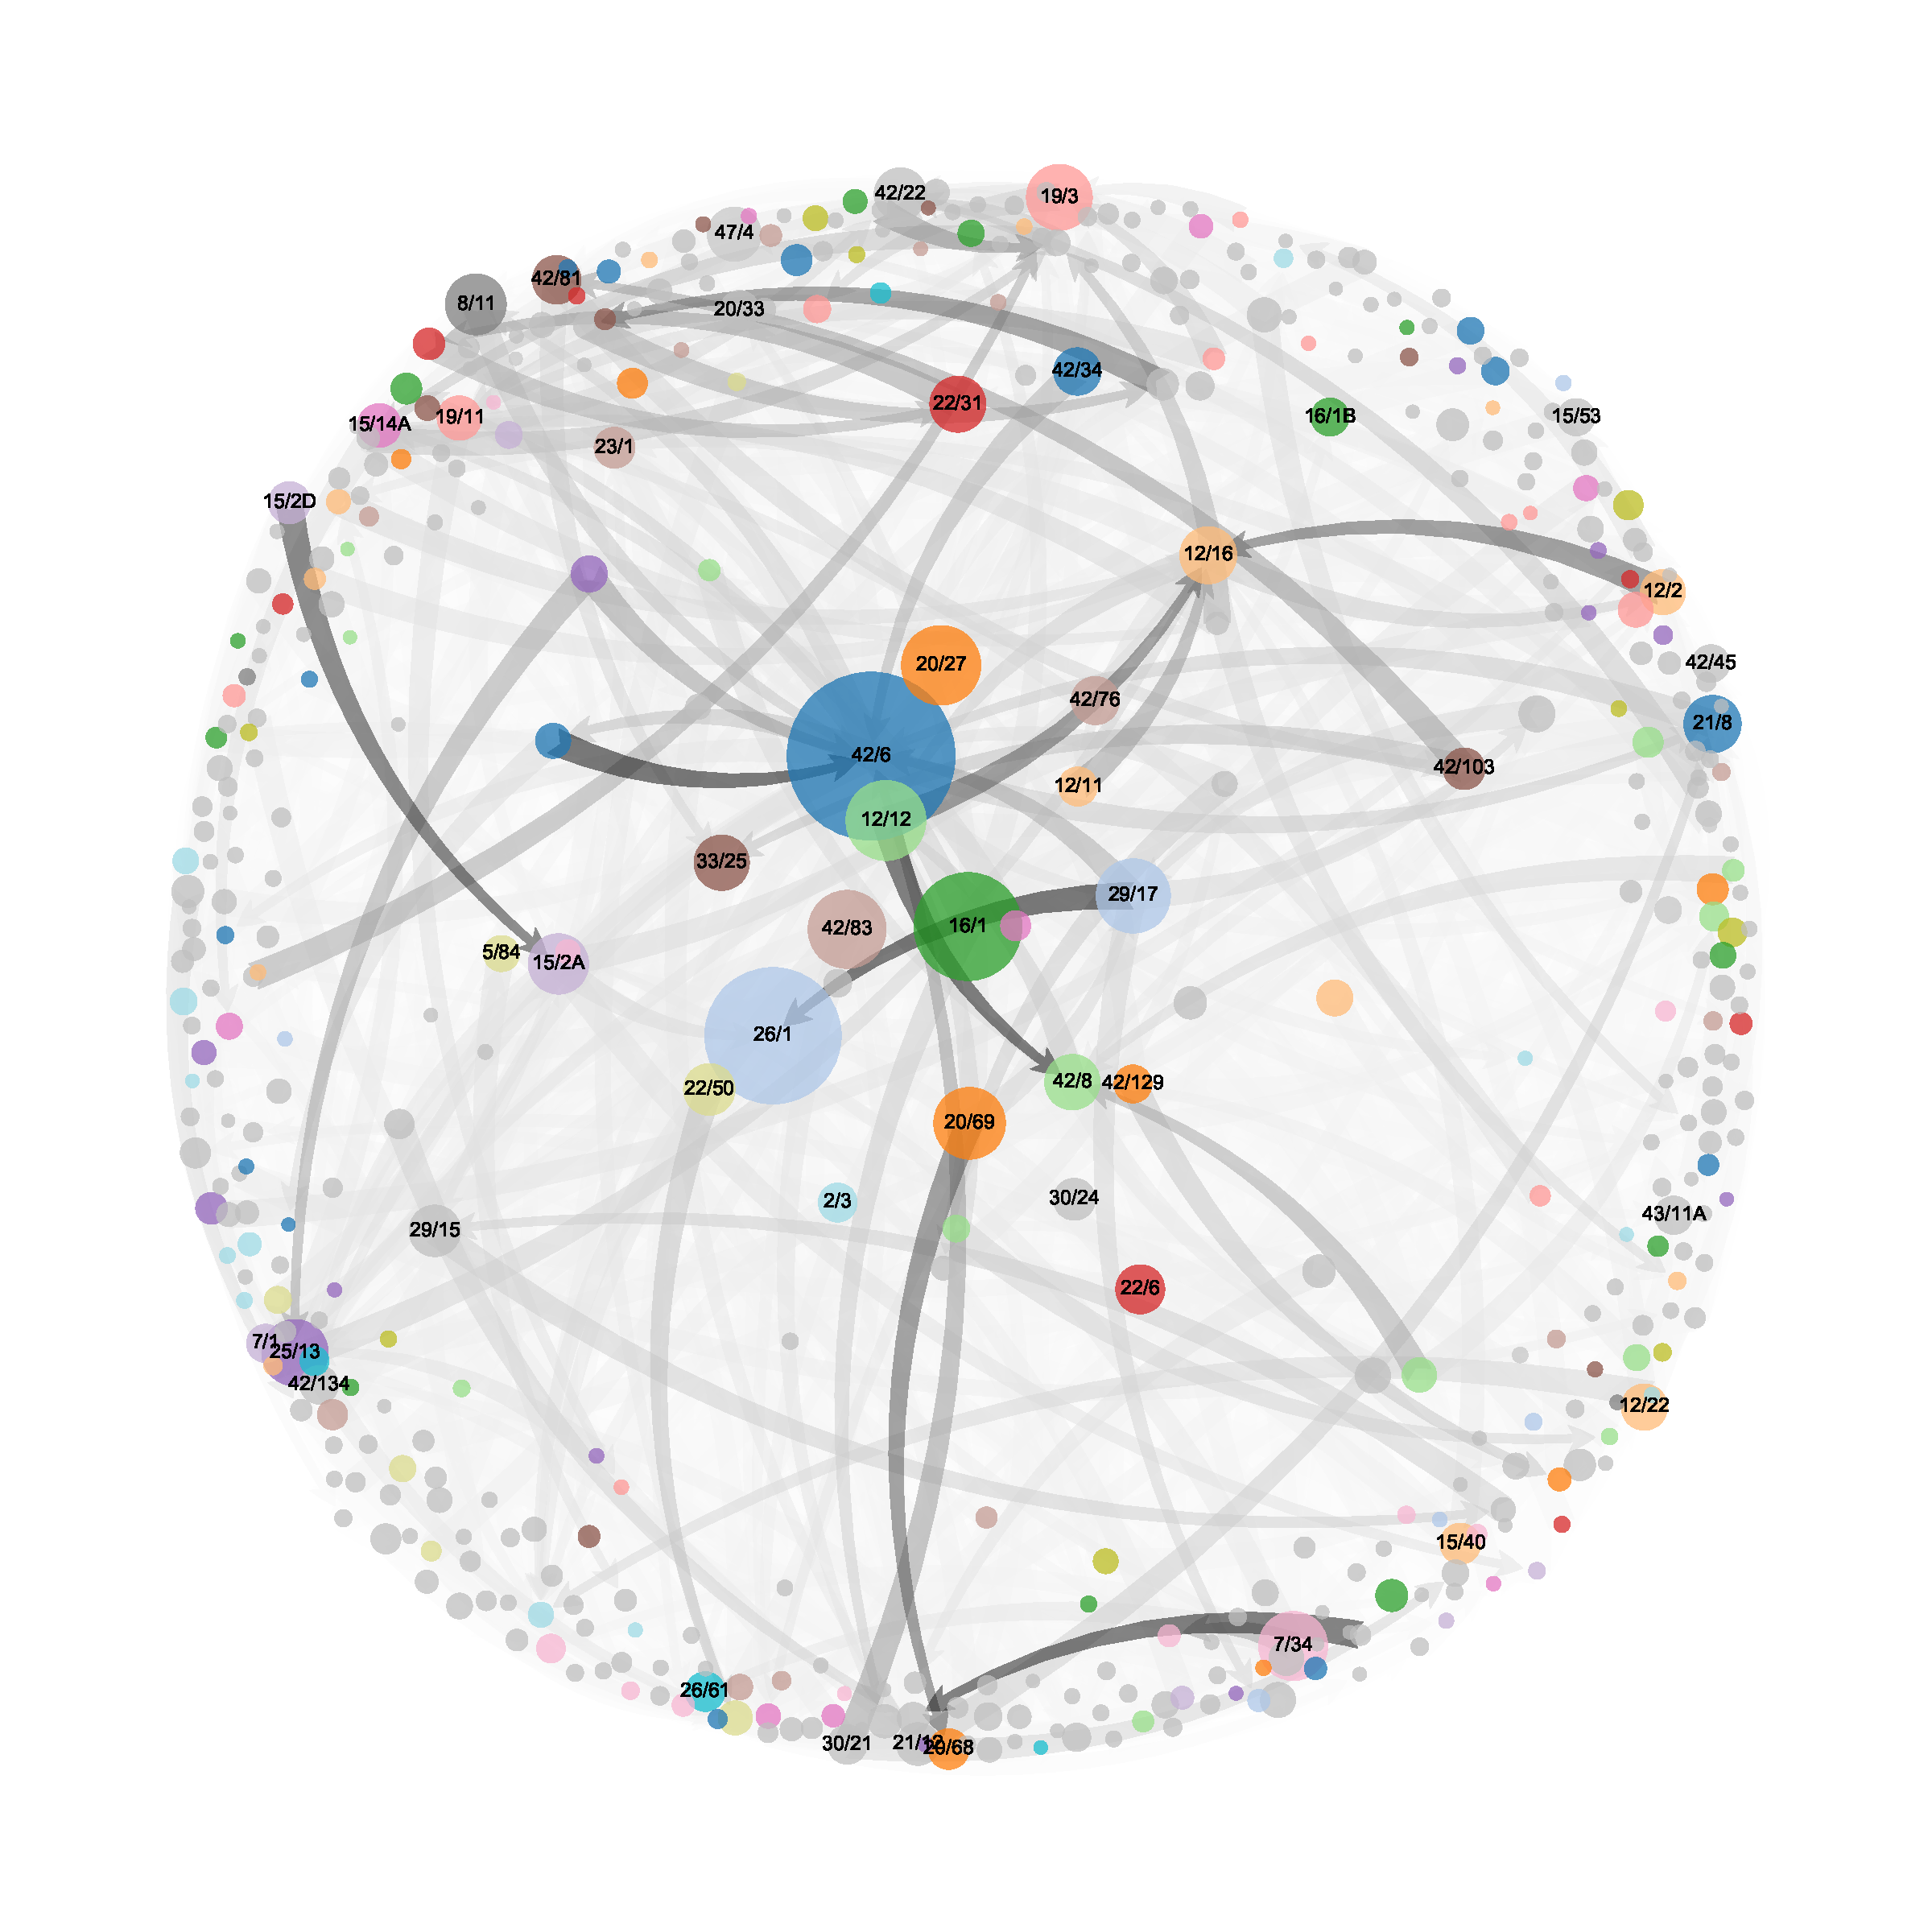
\includegraphics[width=1.085\linewidth]{../../graphics/chapter-graph-1994-us.pdf}~%
	\subcaption{United States (1994)}
\end{subfigure}~%
\begin{subfigure}{0.5\linewidth}
	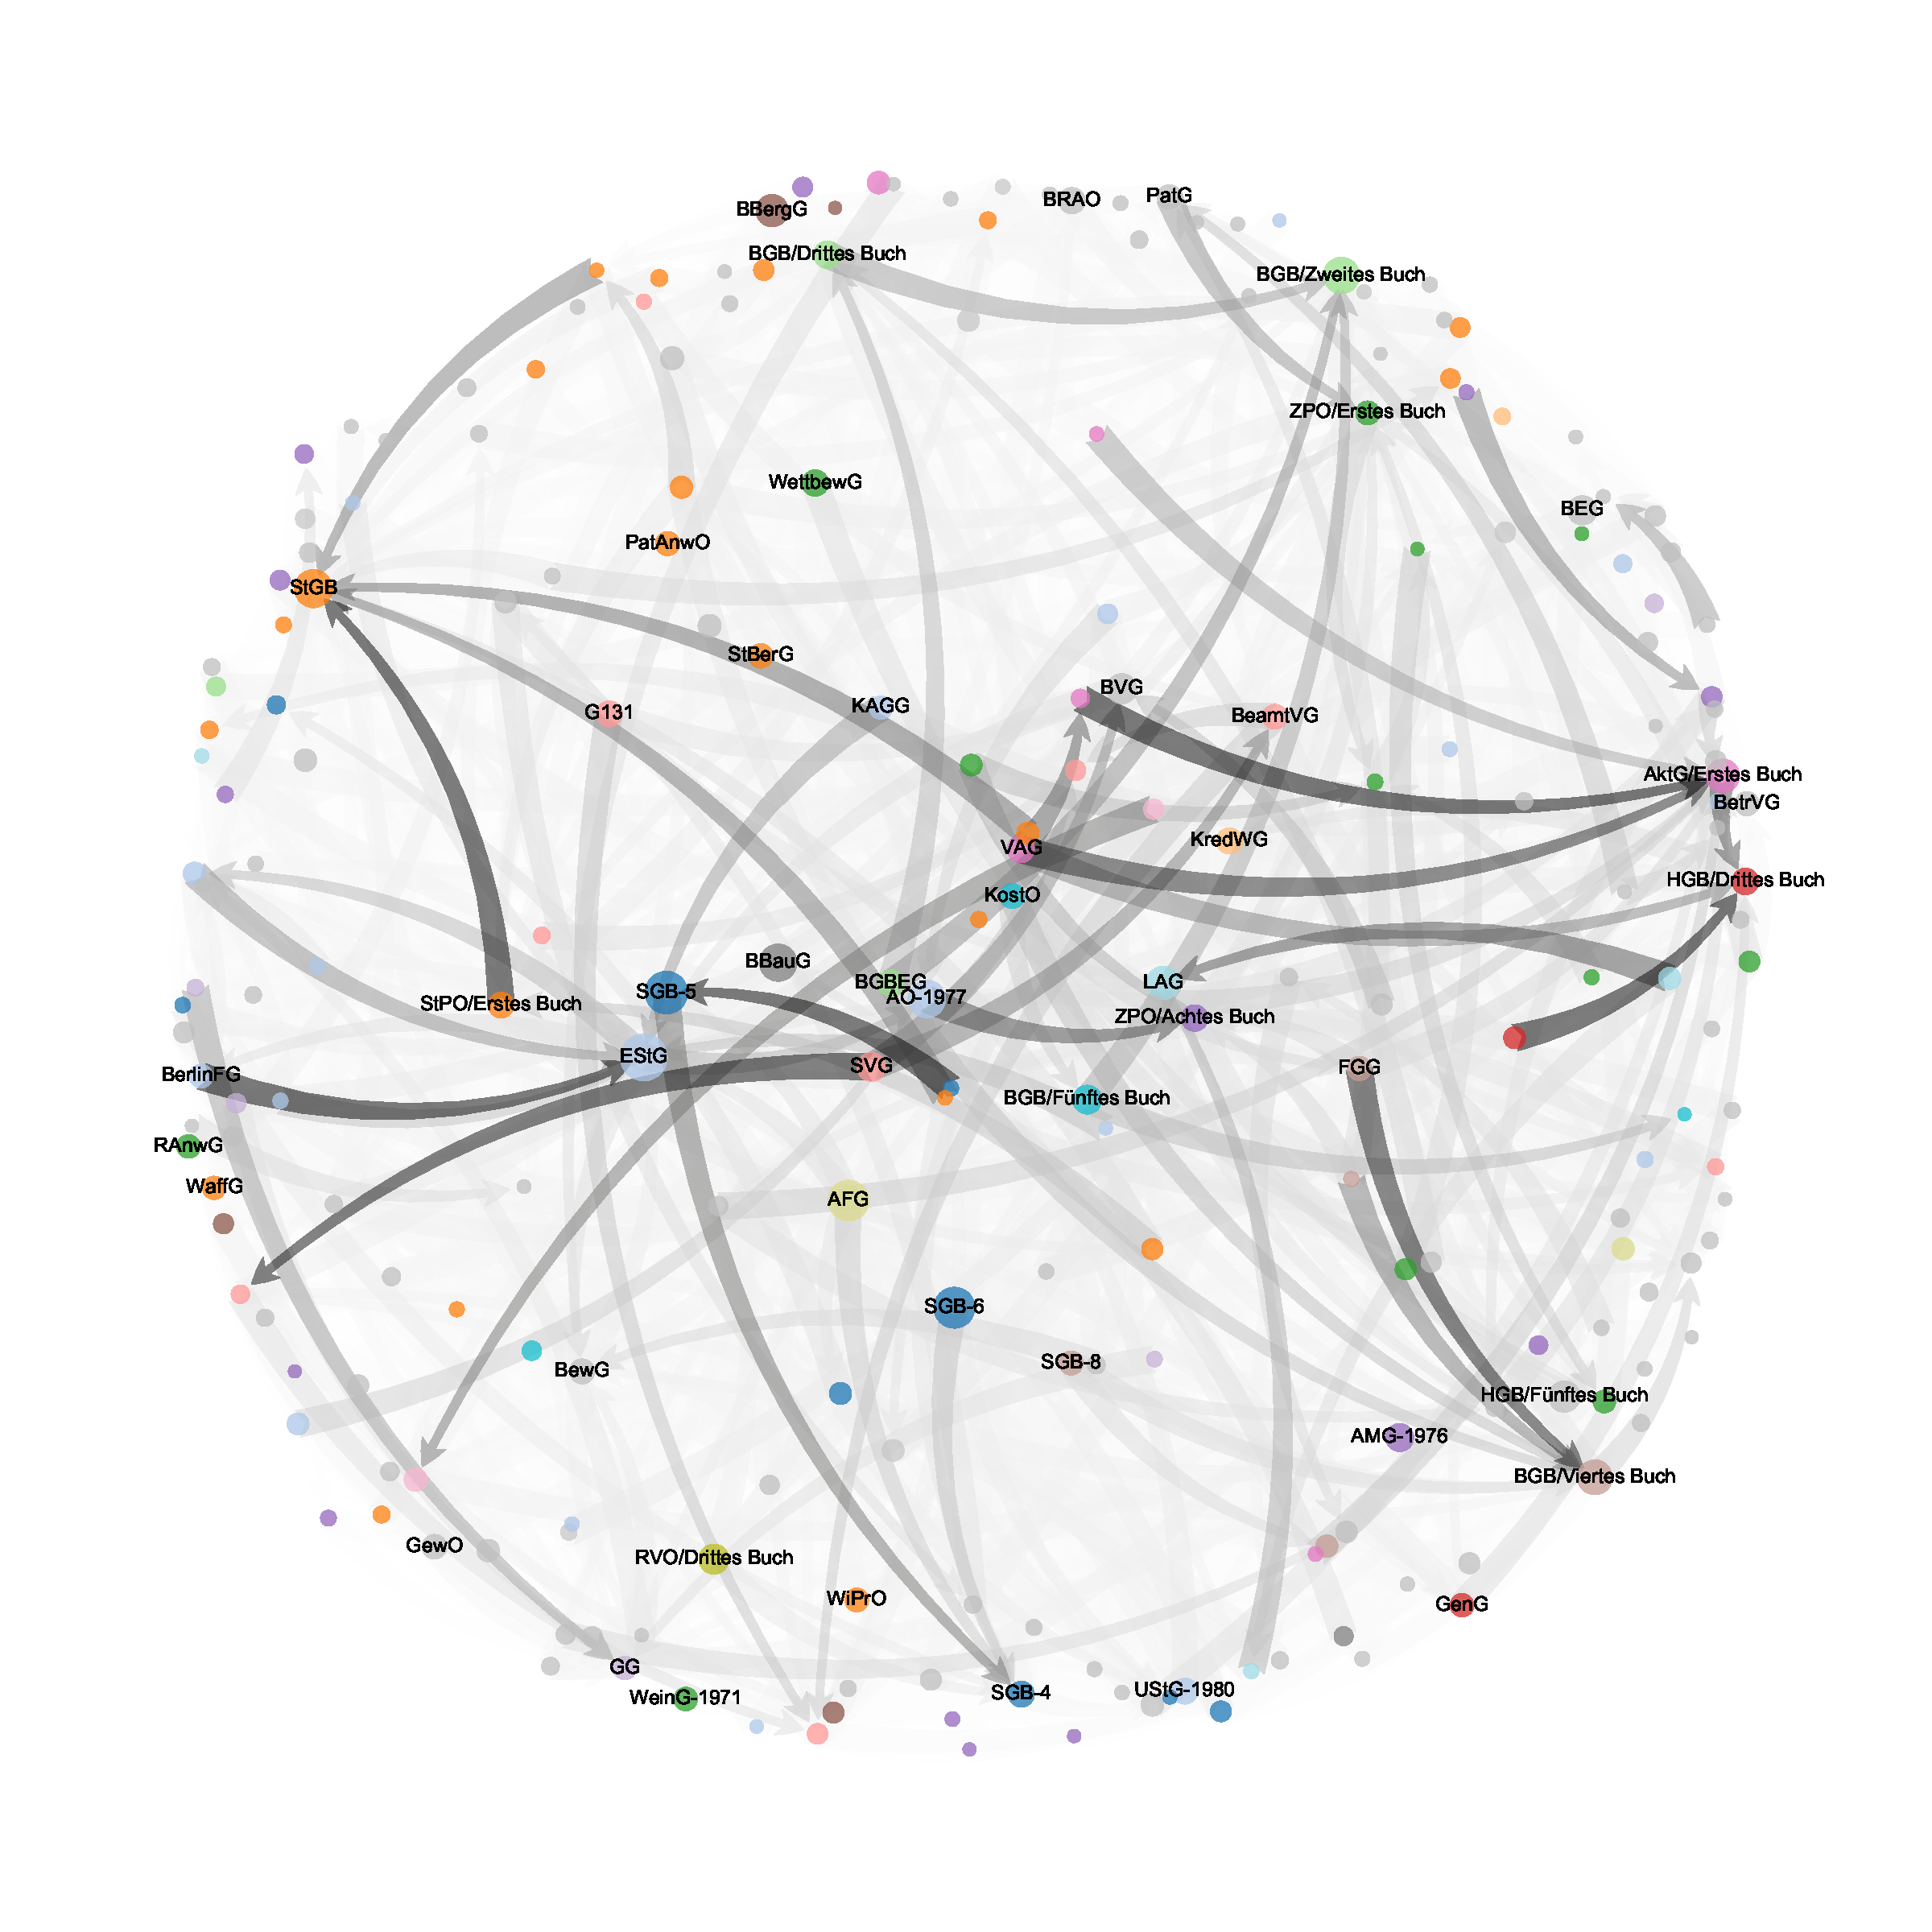
\includegraphics[width=1.085\linewidth]{../../graphics/chapter-graph-1994-de.pdf}~%
	\subcaption{Germany (1994)}
\end{subfigure}
\hspace*{-0.025\linewidth}\begin{subfigure}{0.5\linewidth}
	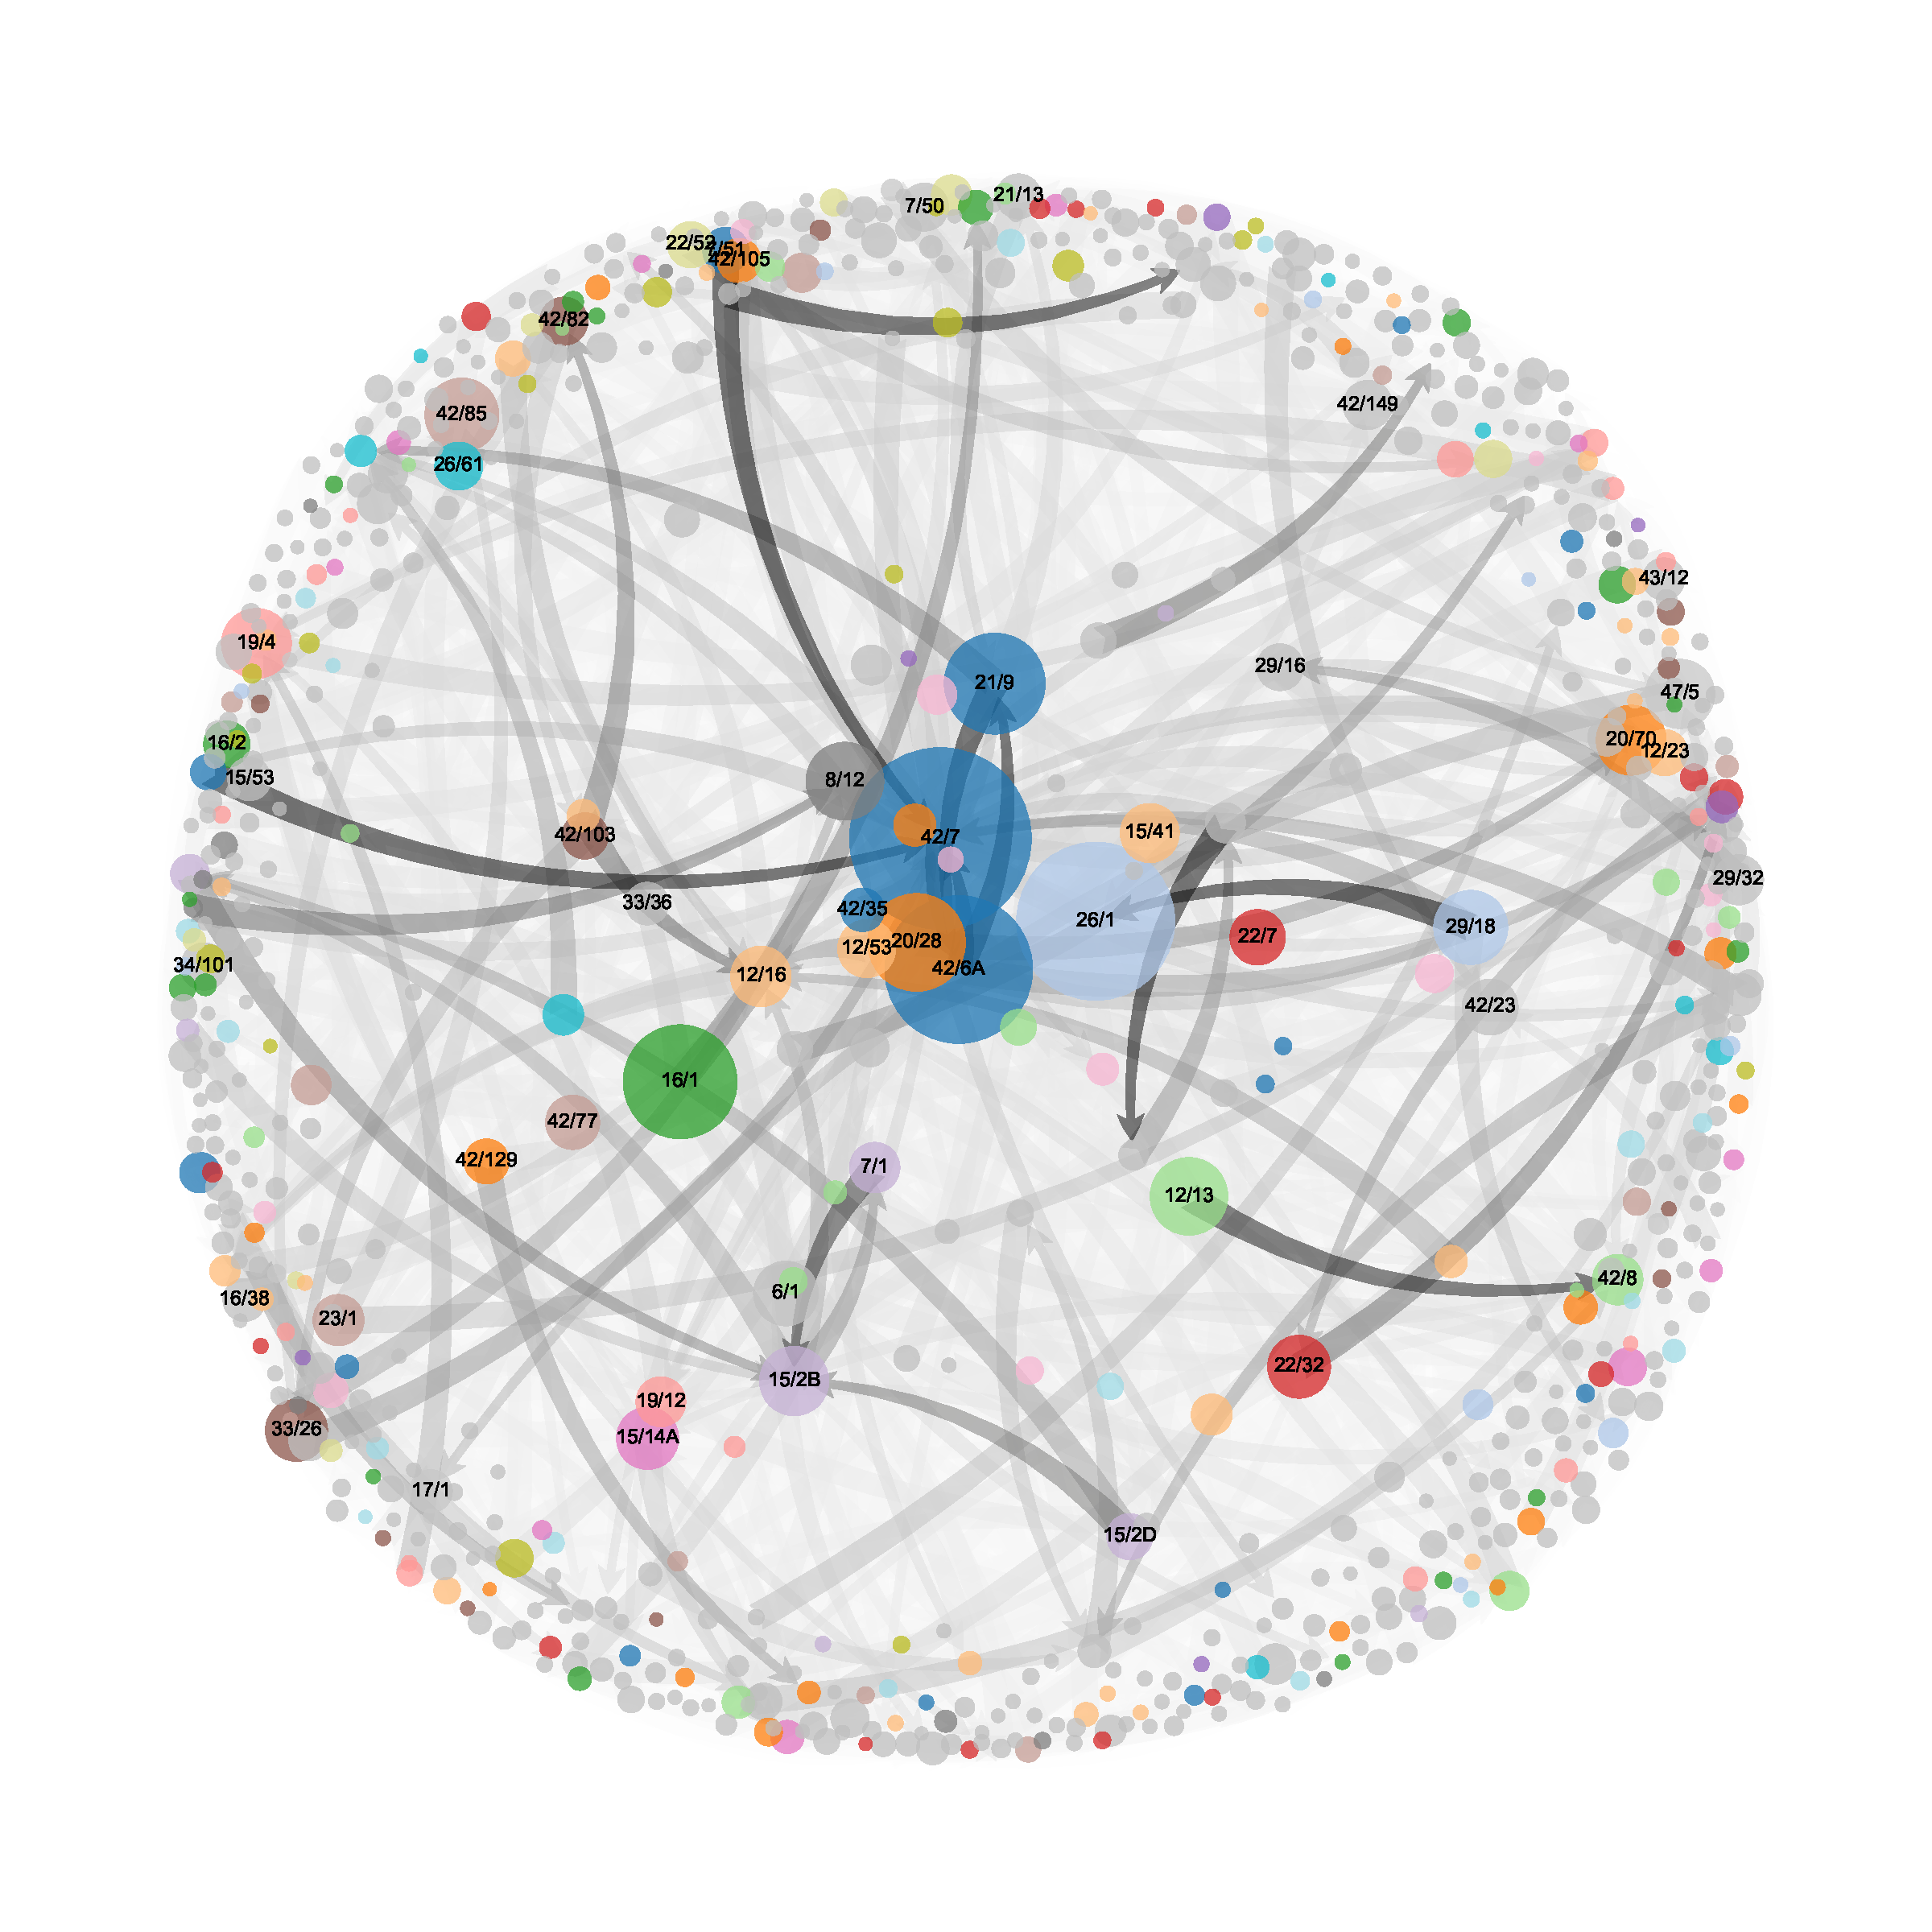
\includegraphics[width=1.085\linewidth]{../../graphics/chapter-graph-2018-us.pdf}~%
	\subcaption{United States (2018)}
\end{subfigure}~%
\begin{subfigure}{0.5\linewidth}
	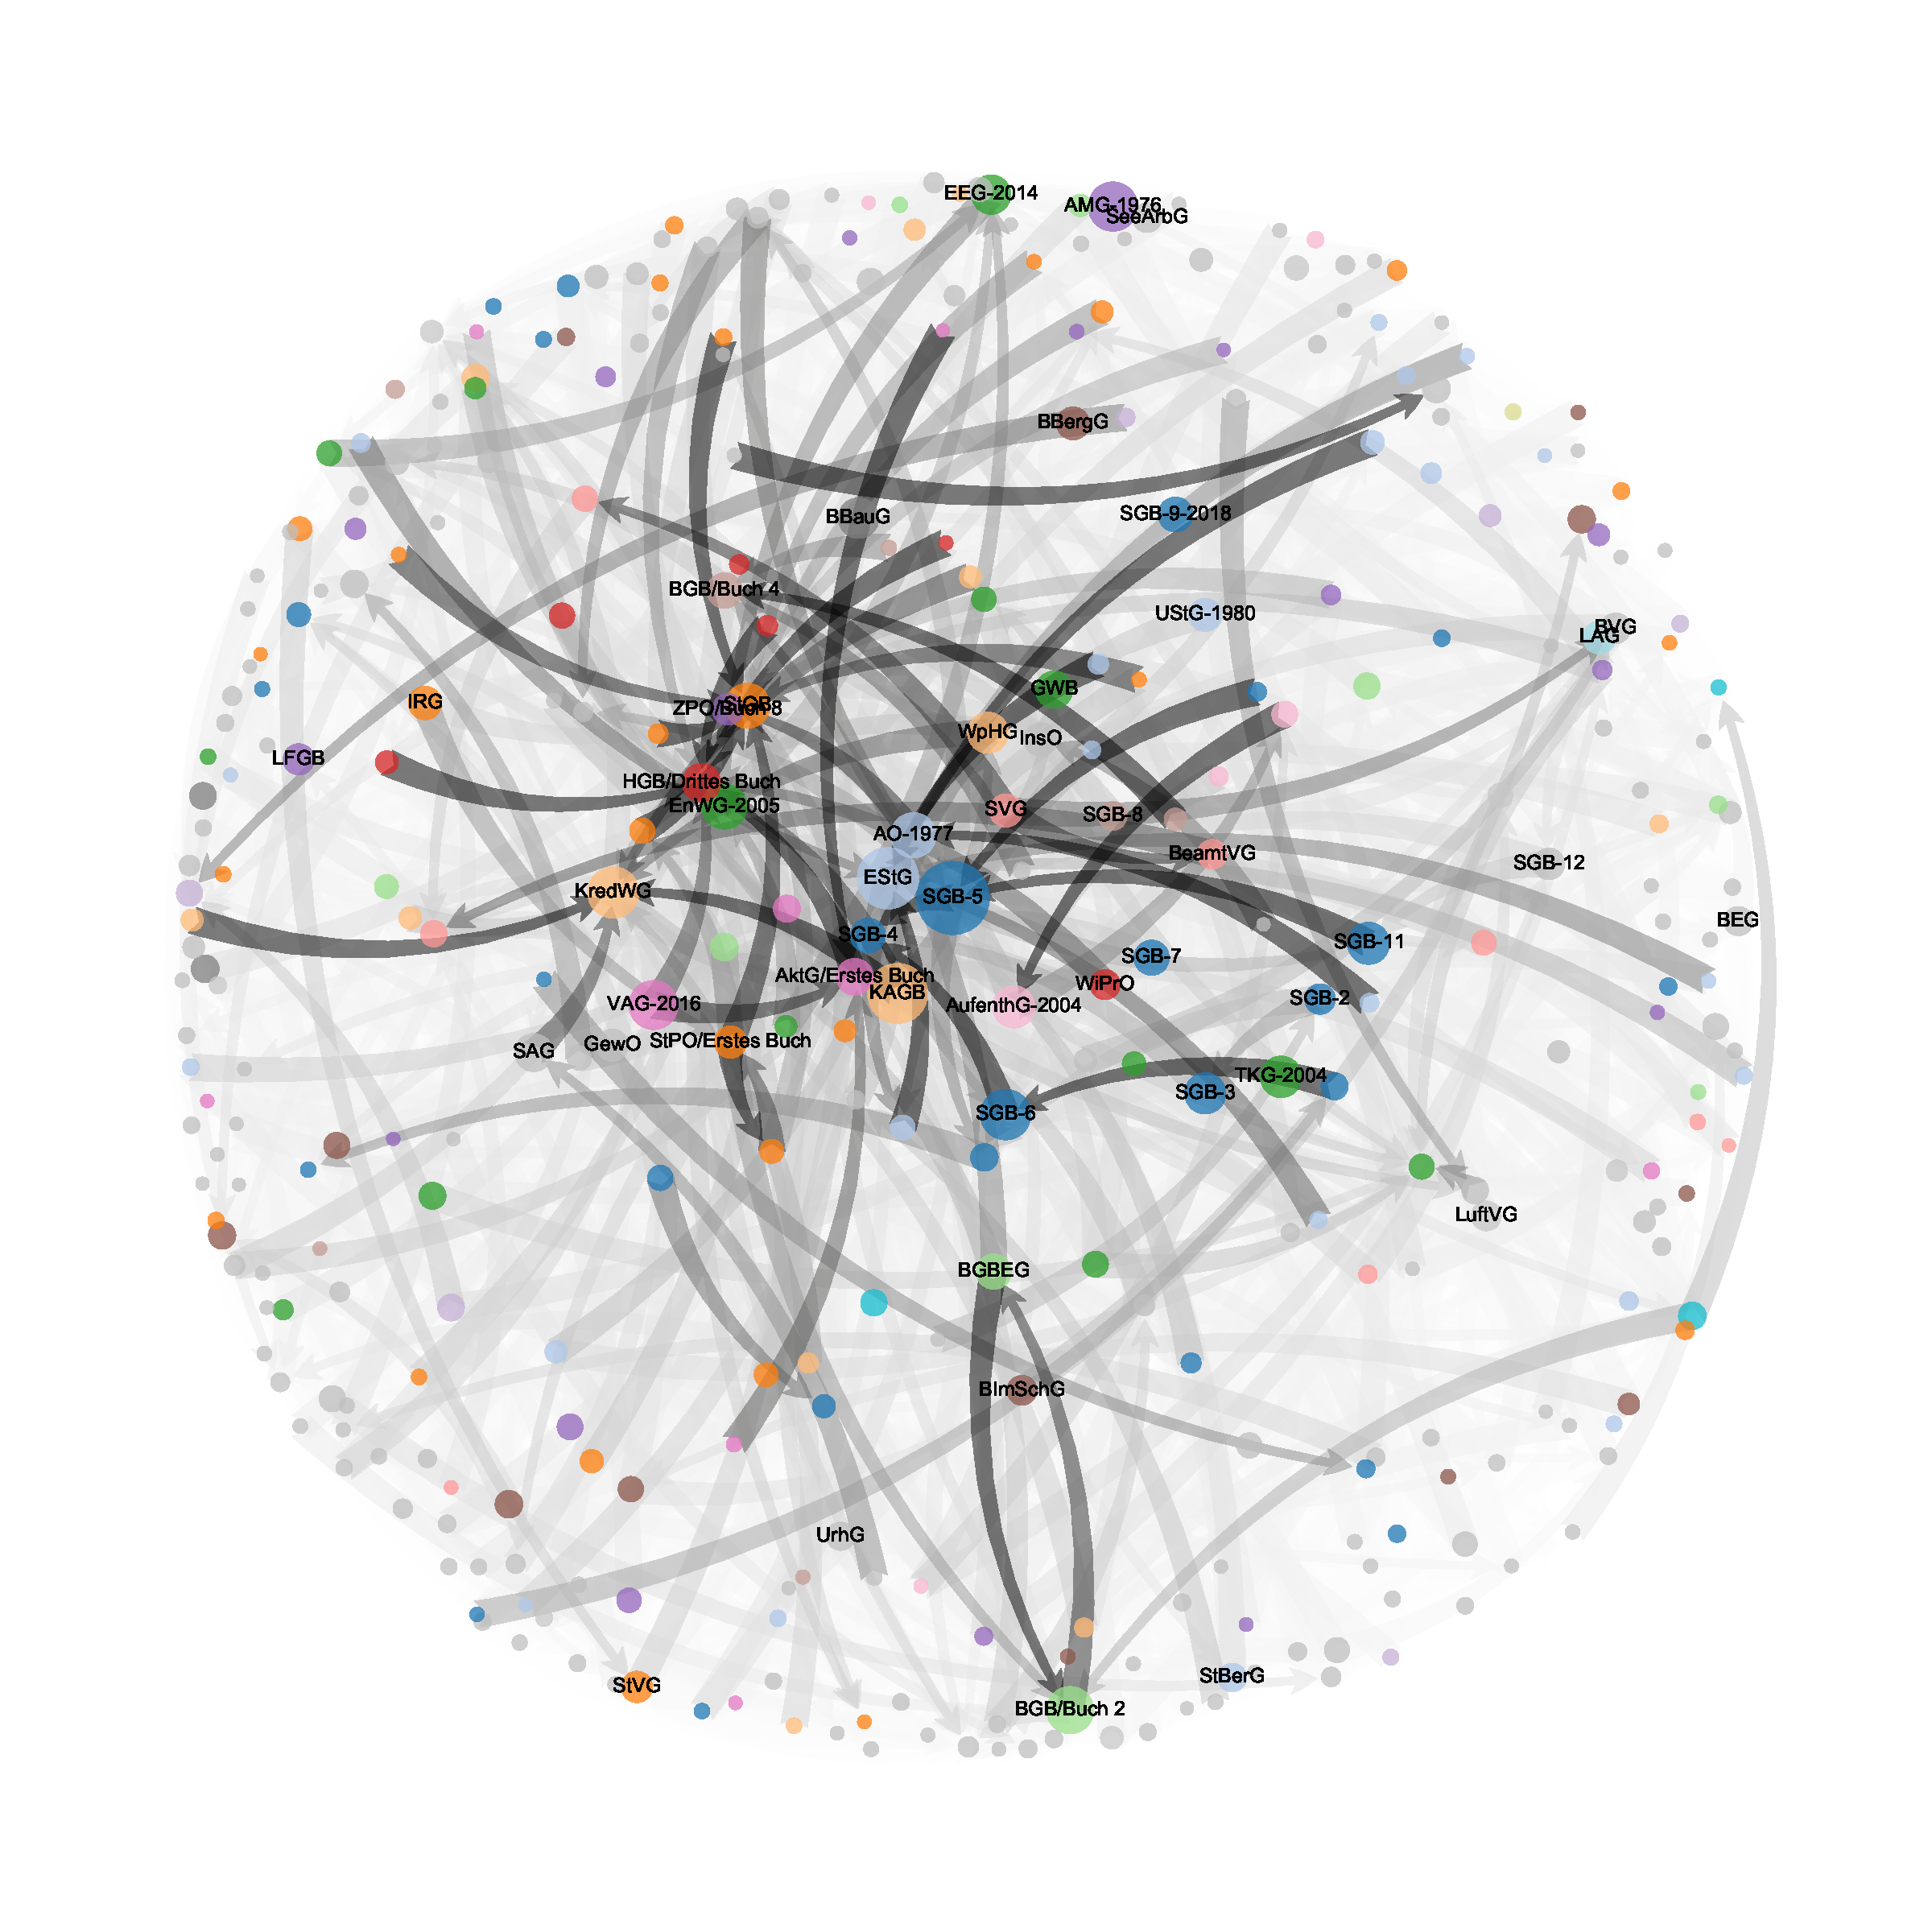
\includegraphics[width=1.085\linewidth]{../../graphics/chapter-graph-2018-de.pdf}~%
	\subcaption{Germany (2018)}
\end{subfigure}
	\end{figure}
	
\end{document}